%!TEX root = ../thesis.tex

\chapter{Implementierung} \label{sec:impl}

%%%%%%%%%%%%%%%%%%%%%%%%%%%%%%%%%%%%%%%%%%%%%%%%%%%%%%%%%%%%%
\section{Architektur \& Moduldesign} 
\label{sec:march}
Die Architektur der VHDL-Implementierung verwendet einen modularen Ansatz. Die zentrale Komponente wird durch den Controller repräsentiert, der den Zustandsautomat, die ECC-, sowie die arithmetischen Operationen beinhaltet und damit die ECDSA-Funktionen (Signieren, Verifizieren)  implementiert. Abbildung \ref{fig:vhdl-impl-arch} zeigt den grundlegenden Aufbau des Systems.   

\begin{figure}[H]
	\centering
  	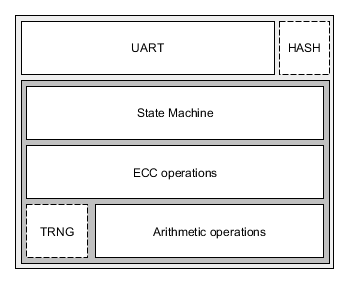
\includegraphics[width=0.7\textwidth]{bilder/vhdl_overview.png}
	\caption{Modulübersicht der FPGA-Hardware. Hauptbestandteil ist der Controller, der den Zustandsautomat, die ECC-, sowie die arithmetischen Operationen beinhaltet. Die Datenübertragung findet über die UART-Schnittstelle statt. Module zum Hashen bzw. zur Zufallszahlengenerierung sind optional und lediglich zur Vollständigkeit erwähnt}
	\label{fig:vhdl-impl-arch}
\end{figure}
 
Die Umschaltung zwischen den verschiedenen Algorithmen findet über einen Zustandsautomat (engl. State Machine) statt. Die Hardware-Implementierung kann zwischen den Modi Signieren und Verifizieren unterschieden. Die Umschaltung findet über die UART-Schnittstelle statt, indem der Datenstrom analysiert wird. Eine detaillierte Beschreibung ist in Abschnitt \ref{sec:uartimpl} zu finden. Je nach gewünschter Funktion, werden andere Parameter über UART empfangen bzw. zurückgeschickt. Eine Übersicht der Parameter beinhaltet Tabelle \ref{tab:vhdl-impl-uart-data}. \\

\begin{table} [h]
	\centering 
	\begin{tabular}{ | p{3cm} | p{2cm} | p{6cm} | }
		\hline
		\textbf{Funktion} & \textbf{Typ} & \textbf{Parameter} \\
		\hline
		Signieren & Input &  Nachricht $m$ (163 Bit) \\
		\hline
		Signieren & Ouput & Signatur $(r,s)$ (326 Bit) \\
		\hline
		Verifizieren & Input & Nachricht $m$ (163 Bit) \\
		\hline
		Verifizieren & Input & Signatur $(r,s)$ (326 Bit) \\
		\hline
		Verifizieren & Output & Ergebnis der Verifizierung (1 Bit) \\
		\hline
	\end{tabular}
	\caption{Eingabe- und Ausgabedaten der VHDL-Implementierung}
	\label{tab:vhdl-impl-uart-data}
\end{table}
 
Wie bereits in Kapitel \ref{sec:ziele} erwähnt, wurde auf eine sicherheitsorientierte Implementierung des Algorithmus verzichtet, sodass anstatt eines ``echten'' Zufallszahlengenerators  (engl. True Random Number Generator, TRNG), lediglich eine festgelegte Konstante zum Einsatz kommt. Hauptgrund für diese Entscheidung begründet sich mit der fehlenden Hardware zum Generieren einer sicheren Zufallszahl. Als eine weitere Vereinfachung wurde auf eine Einheit zum Generieren eines Hashes verzichtet, um den Fokus auf die Implementierung der ECC-Operationen zu lenken, ohne die Messergebnisse durch die HASH-Generierung zu verfälschen. Aus Gründen der Vollständigkeit sind beide Komponenten dennoch in Abbildung \ref{fig:vhdl-impl-arch} zu finden. 

%%%%%%%%%%%%%%%%%%%%%%%%%%%%%%%%%%%%%%%%%%%%%%%%%%%%%%%%%%%%%

\section{Parameter}
\label{vhdl-impl-parameter}

Die gesamte VHDL-Implementierung setzt ausschließlich auf VHDL-typische Generics. Diese werden über das globale Paket \texttt{tld\_ecdsa\_package} verwaltet. Neben den Parametern enthält das Paket globale Hilfsfunktionen, die zum Beispiel eine Matrix-Reduktion durchführen. Tabelle \ref{tab:vhdl-impl-param} zeigt eine Übersicht der wichtigsten Parameter.

\begin{table} [h]
	\centering 
	\begin{tabular}{ | p{3cm} | p{12cm} | }
		\hline
		\textbf{Parameter} & \textbf{Beschreibung}\\
		\hline
		M & Bitbreite des Schlüssels bzw. der Daten (z.B. 163) \\
		\hline
		N & Modolo-Parameter der Kurve (Bestandteil des ECDSA-Algorithmus) \\
		\hline
		P & Anzahl der Elemente im GF($2^M$) \\
		\hline
		BAUD\_RATE & Eingestellte Baud-Rate der UART-Schnittstelle \\
		\hline
	\end{tabular}
	\caption{Parameter der VHDL-Implementierung}
	\label{tab:vhdl-impl-param}
\end{table}

Von Vorteil ist, dass durch den Einsatz dieses Pakets möglich ist, Parameter zu ändern, um beispielsweise eine andere Schlüssellänge oder Kurvenparameter zu verwenden. Ein Nachteil dagegen ist, dass durch die generische Implementierung weniger Spielraum für Performance-Optimierung besteht. 


%%%%%%%%%%%%%%%%%%%%%%%%%%%%%%%%%%%%%%%%%%%%%%%%%%%%%%%%%%%%%

\section{Top-Level-Entität}
\label{vhdl-impl-tld}

Wie bereits erwähnt kommuniziert die Top-Level-Entität über eine serielle RS232-Schnittstelle mit einem Computer oder einem anderen Gerät, um Daten auszutauschen. Dazu werden lediglich zwei Pins zur UART-Kommunikation, sowie ein globales 50Mhz-Takt- und Resetsignal benötigt. Abbildung \ref{fig:pins} zeigt die genaue Zuordnung der Pins auf dem FPGA. 

\begin{figure}[H]
	\centering
	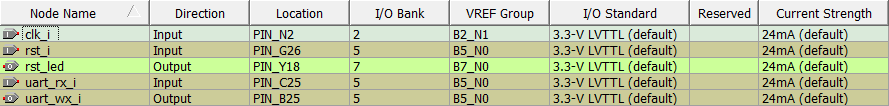
\includegraphics[width=\textwidth]{bilder/pins}
	\caption{Pin-Zuordnung des FPGA}
	\label{fig:pins}
\end{figure}

Nach vollständigem Erhalt der Daten, die sich je nach Algorithmus unterscheiden (vgl. Tabelle \ref{tab:vhdl-impl-uart-data}), werden diese dem zentralen Modul \texttt{e\_ecdsa} bereitgestellt. Über binäre Eingänge wird festgelegt, welcher Modus (Signieren vs. Verifizieren, Pin \texttt{mode\_i}) verwendet und wann die Berechnung gestartet werden soll (Pin \texttt{enable\_i}).
 
\begin{figure}[thb]
	\centering
	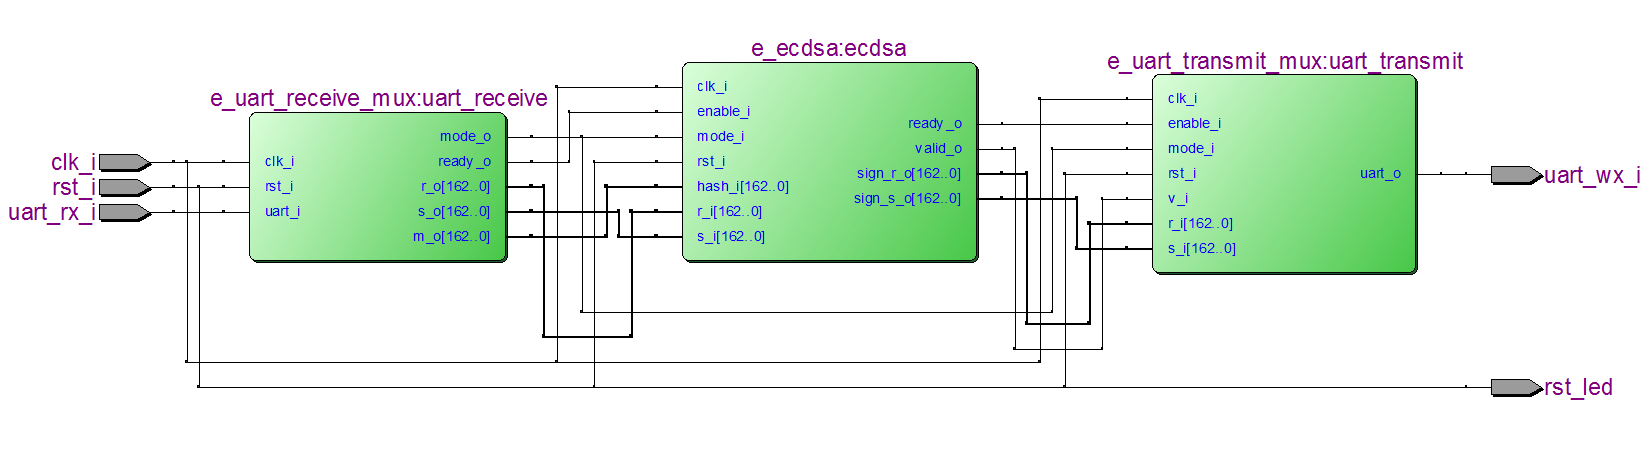
\includegraphics[width=\textwidth]{bilder/tle}
	\caption{Top-Level-Entity der VHDL-Implementierung}
	\label{fig:vhdl-impl-tle}
\end{figure}

Sobald die ECDSA-Entität die Berechnung abgeschlossen hat, wird ein binäres Flag gesetzt, sodass die Daten über das Modul \texttt{e\_uart\_transmit\_mux} zurückschickt.  

\begin{table} [h]
	\centering 
	\begin{tabular}{ | p{3cm} | p{12cm} | }
		\hline
		\textbf{Parameter} & \textbf{Beschreibung}\\
		\hline
		clk\_i & Globales Taktsignal \\
		\hline
		rst\_i & Resetsignal \\
		\hline
		uart\_rx\_i & Pin zum Lesen der UART-Kommunikation \\
		\hline
		uart\_tx\_i & Pin zum Schreiben der UART-Kommunikation \\
		\hline
		rst\_led & LED zur Kennzeichnung ob das Reset-Signal aktiv ist \\
		\hline
	\end{tabular}
	\caption{Eingabe- und Ausgabeparameter der Haupt-Entität}
	\label{tab:vhdl-impl-tld-ecdsa-param}
\end{table}


%%%%%%%%%%%%%%%%%%%%%%%%%%%%%%%%%%%%%%%%%%%%%%%%%%%%%%%%%%%%%
\section{ECDSA-Implementierung}
\label{vhdl-impl-general}

Die ECDSA-Implementierung verwendet zum Umschalten zwischen Signieren und Verfifizieren einen Zustandsautomat, der im wesentlichen im Abhängigkeit des Parameters \texttt{mode\_i} zwischen den Algorithmen wechselt. 

\begin{figure}[thb]
	\centering
	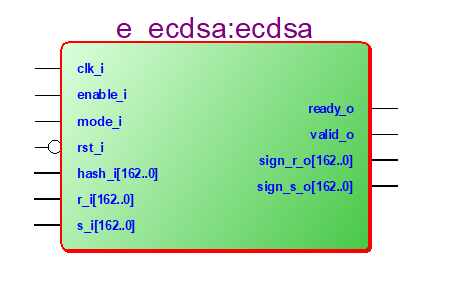
\includegraphics[width=0.5\textwidth]{bilder/e_ecdsa.png}
	\caption{ECDSA-Entität}
	\label{fig:vhdl-impl-e_ecdsa}
\end{figure}

Die Implementierungen der Algorithmen folgt dem Ablauf aus Kapitel \ref{ecdsa-algo}. Jeder Teil des Algorithmus, sei es eine klassische arithmetische oder elliptische Operation, wird über eine separate VHDL-Entität repräsentiert. Der Ablauf ist streng sequentiell, wobei versucht wird, einen maximalen Parallelisierungsgrad anzustreben. So werden bei der Verifikation beispielsweise die Variablen $u_1$ und $u_2$ parallel berechnet.
\\ \\
Jede Entität verfügt über ein Flag zur Aktivierung und ein Flag welches kennzeichnet, ob die Berechnung abgeschlossen ist. Das Abfragen bzw. Aktivieren der Flags wird über den Zustandsautomat realisiert.

\begin{table} [h]
	\centering 
	\begin{tabular}{ | p{3cm} | p{12cm} | }
		\hline
		\textbf{Parameter} & \textbf{Beschreibung}\\
		\hline
		clk\_i & Globales Taktsignal \\
		\hline
		rst\_i & Resetsignal \\
		\hline
		enable\_i & Flag zum Aktivieren der Berechnung \\
		\hline
		mode\_i & Flag zum Umschalten zwischen Signieren und Verifizieren \\
		\hline
		hash\_i & Eingabe Text \\
		\hline
		r\_i & R-Komponente der zu verifizierenden Signatur \\
		\hline
		s\_i & S-Komponente der zu verifizierenden Signatur \\
		\hline
		ready\_o & Status-Flag ob die Berechnung abgeschlossen ist  \\
		\hline
		valid\_o & Flag ob die zu verifizierenden Signatur valide ist \\
		\hline
		r\_o & R-Komponente der erstellten Signatur \\
		\hline
		s\_s & S-Komponente der erstellten Signatur \\
		\hline
	\end{tabular}
	\caption{Eingabe- und Ausgabeparameter der ECDSA-Entität}
	\label{tab:vhdl-impl-ecdsa-param}
\end{table}

\subsection{Punkt-Multiplikation}

\subsection{Punkt-Addition}

\subsection{Punkt-Dopplung}

\subsection{Addierer}

\subsection{Multiplizierer}

\subsection{Dividierer}

\subsection{Invertierer}

\subsection{Quadrierer}



%%%%%%%%%%%%%%%%%%%%%%%%%%%%%%%%%%%%%%%%%%%%%%%%%%%%%%%%%%%%%
\section{Kommunikation der UART-Verbindung} \label{sec:uartimpl}

Die UART-Komponenten übernehmen wie in Kap. \ref{sec:iuart} beschrieben neben der externen Kommunikation auch die Transformation der Daten. Dabei wird der Rx-Input\footnote{Das Rx-Signal wird erst nach Einsynchronisation mit zwei aufeinanderfolgenden Flip-Flops verarbeitet.} nach dem Empfangen über Register mit einem Parallel-Ausgang zur Verfügung gestellt. Abbildung \ref{fig:uartrx} zeigt die Verschaltung des \textbf{Receivers} mit den Schieberegistern im RTL Viewer der Entwicklungsumgebung. \\

\begin{figure}[thb]
	\centering
  	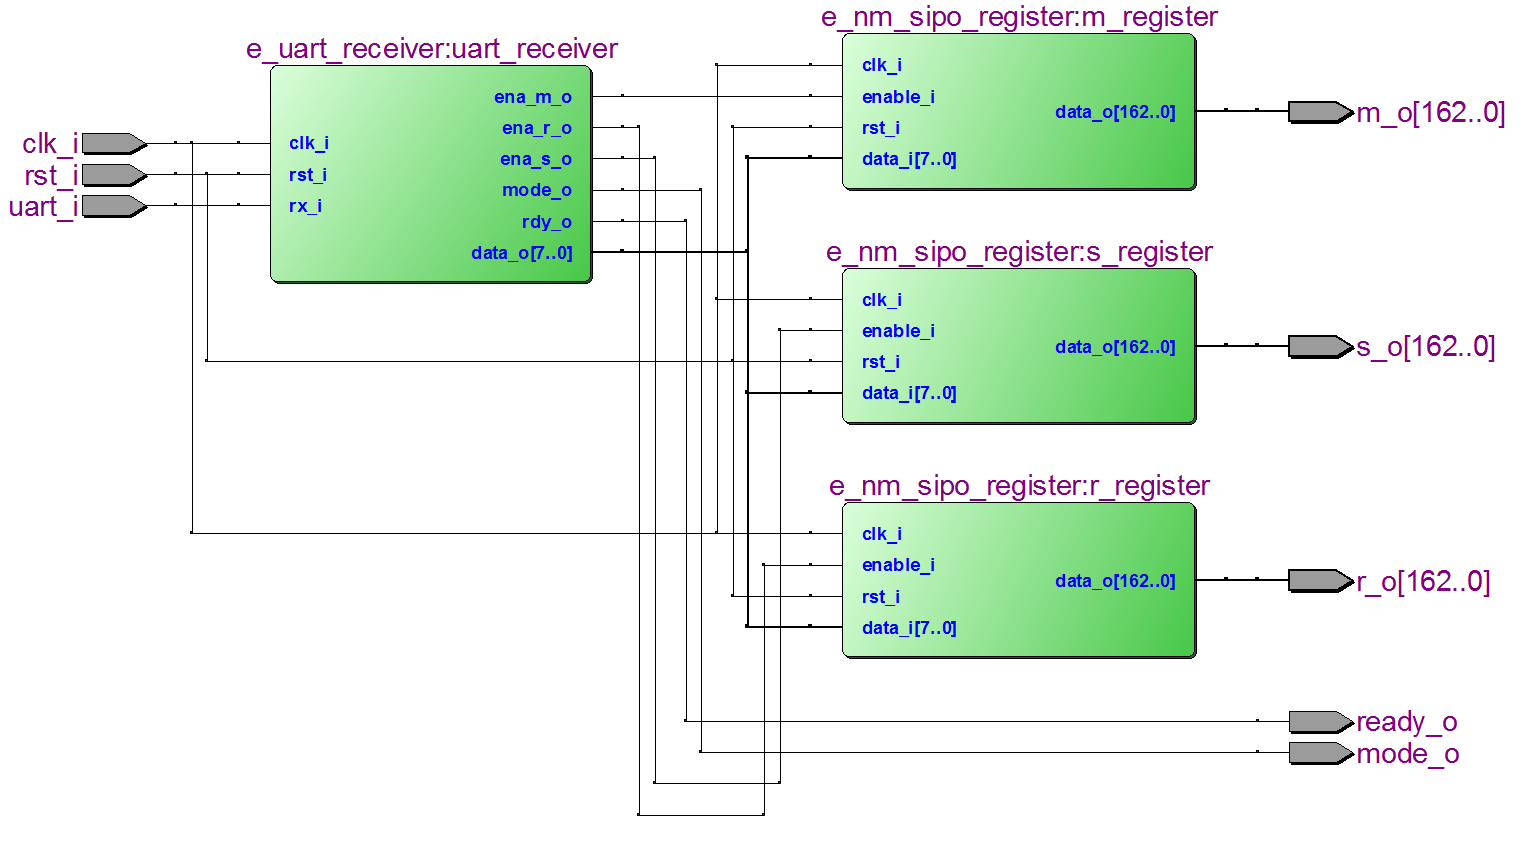
\includegraphics[width=0.9\textwidth]{bilder/uart-receiver}
	\caption{Ansicht des UART-Receivers im RTL Viewer}
	\label{fig:uartrx}
\end{figure}

Der Receiver selbst enthält einen Zustandsautomaten, der den Eingabedatenstrom in die zwei Modi \texttt{Signieren} und \texttt{Verifizieren} klassifiziert. Anhand der Zustände werden die Steuerungssignale am Modulausgang (\textit{enable}-Signale für die Punkte $r$ und $s$ auf der elliptischen Kurve sowie die Nachricht) so geschaltet, sodass jeweils die entsprechenden Eingabewörter in den dafür vorgesehenen Registern landen\footnote{phase1 = $r$, phase2 = $s$, phase3 = $message$} (vgl. Abb. \ref{fig:uart-receiver-phase}. Hierfür gibt es zwei vorangegangene Phase, in denen der Modus durch das erste empfangene Byte bestimmt wird (\textit{dmode}) und anschließend über die Dauer eines Taktzyklus umgeschaltet wird (\textit{smode}). \\

\begin{figure}[thb]
	\centering
  	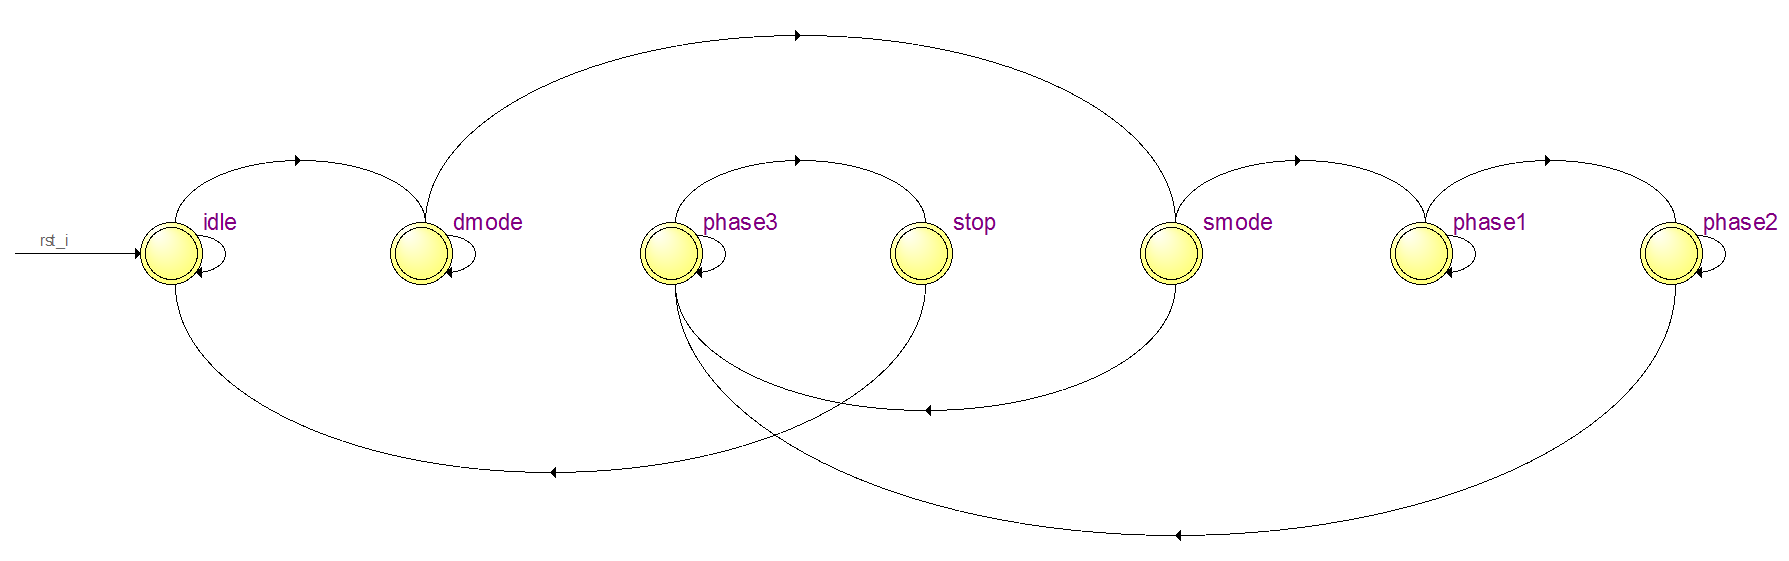
\includegraphics[width=\textwidth]{bilder/uart-receiver-phase}
	\caption{Zustandsautomat des Receivers zu Phasen-Bestimmung beim Empfang}
	\label{fig:uart-receiver-phase}
\end{figure}

Die Phasen des gezeigten Automaten bilden eine Abstraktionsebene über der eigentlichen Erkennung der sequentiellen Datenbits am Rx-Eingang. Ein weiterer Zustandsautomat (s. Anhang \ref{fig:uart-receiver-data}) agiert innerhalb eines UART-Datenpaketes (Start-Bit, 8 Bit Daten, Stop-Bit) und speichert ein einzelnes Byte zwischen zur Weiterverarbeitung. Der erste Byte für den Modus muss dabei entweder ``00000000b'' für das Signieren oder ``11111111b'' für das Verifizieren sein. Der Modus wird als binäres Signal für nachfolgende Module nach außen geführt. \\

Der \textbf{UART-Transmitter} beinhaltet zwei Schieberegister, die einen parallelen Eingang mit einem Byte-weise seriellen Ausgang besitzen (vgl. Abb. \ref{fig:uarttx}). Das \texttt{e\_uart\_transmit}-Modul steuert diese Register über einen internen Zustandsautomaten gibt die entsprechenden Steuerungssignale nach außen an die beiden Multiplexer, welche die \textit{enable}-Eingänge anspricht. \\

\begin{figure}[H]
	\centering
  	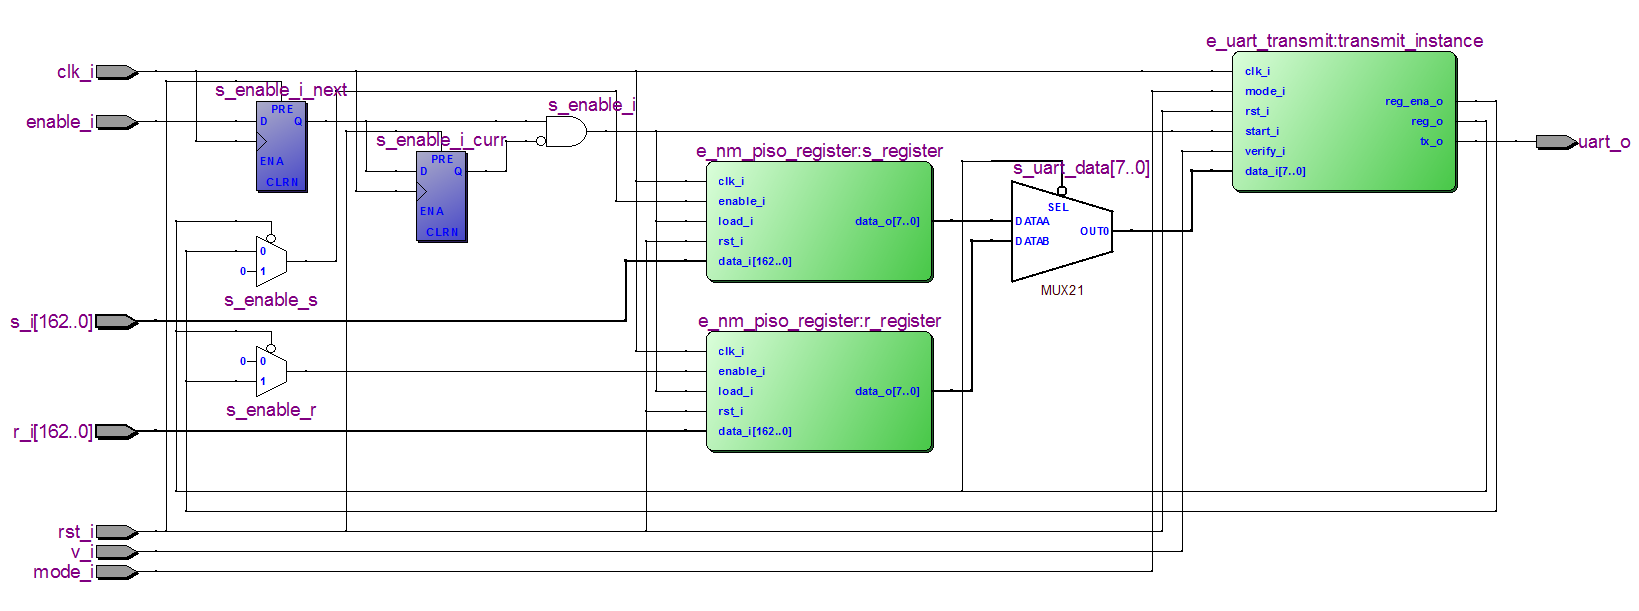
\includegraphics[width=\textwidth]{bilder/uart-transmitter}
	\caption{Ansicht des UART-Transmitter im RTL Viewer}
	\label{fig:uarttx}
\end{figure}

Im Modus Signieren sendet das Modul den in den Registern gespeicherten Punkt $(r, s)$. Beim Verifizieren wird entweder ein Byte Nullen (Signatur passt \textit{nicht} zum Dokument) oder ein Byte Einsen (Signatur gehört zum Dokument) versendet. Der Transmitter instantiiert intern einen Timer, der das Senden am Ausgang Tx in der vor der Synthetisierung eingestellten Baud-Rate taktet. \\



%%%%%%%%%%%%%%%%%%%%%%%%%%%%%%%%%%%%%%%%%%%%%%%%%%%%%%%%%%%%%
\section{Synthetisierungsergebnisse}

Der verwendete FPGA ist ein Baustein der Altera Cyclone II Familie (EP2C35F672C6). Für die Synthetisierung wird das in der Entwicklungsumgebung Quartus II vom selben Hersteller enthaltene Werkzeug verwendet. \\

\begin{table} [h]
	\centering 
	\begin{tabular}{ | p{6cm} | p{3cm} | }
		\hline
		\textbf{Beschreibung} & \textbf{Wert}\\
		\hline
		Ressourcennutzung & 21\% \\
		\hline
		Anzahl Logikelemente & 23097 \\
		\hline
		Anzahl Register & 15508 \\
		\hline
		Anzahl Pins & 5 \\
		\hline
	\end{tabular}
	\caption{Ergebnisse der Synthetisierung}
	\label{tab:vhdl-impl-de2}
\end{table}

